%%%%%%%%%%%%%%%%%%%%%%%%%%% asme2ej.tex %%%%%%%%%%%%%%%%%%%%%%%%%%%%%%%
% Template for producing ASME-format journal articles using LaTeX    %
% Written by   Harry H. Cheng, Professor and Director                %
%              Integration Engineering Laboratory                    %
%              Department of Mechanical and Aeronautical Engineering %
%              University of California                              %
%              Davis, CA 95616                                       %
%              Tel: (530) 752-5020 (office)                          %
%                   (530) 752-1028 (lab)                             %
%              Fax: (530) 752-4158                                   %
%              Email: hhcheng@ucdavis.edu                            %
%              WWW:   http://iel.ucdavis.edu/people/cheng.html       %
%              May 7, 1994                                           %
% Modified: February 16, 2001 by Harry H. Cheng                      %
% Modified: January  01, 2003 by Geoffrey R. Shiflett                %
% Use at your own risk, send complaints to /dev/null                 %
%%%%%%%%%%%%%%%%%%%%%%%%%%%%%%%%%%%%%%%%%%%%%%%%%%%%%%%%%%%%%%%%%%%%%%

%%% use twocolumn and 10pt options with the asme2ej format
\documentclass[twocolumn,10pt]{asme2ej}

\usepackage{epsfig} %% for loading postscript figures
\usepackage[T1]{fontenc}
\usepackage{lipsum}% http://ctan.org/pkg/lipsum
\usepackage{graphicx}% http://ctan.org/pkg/graphicx
% ....


%% The class has several options
%  onecolumn/twocolumn - format for one or two columns per page
%  10pt/11pt/12pt - use 10, 11, or 12 point font
%  oneside/twoside - format for oneside/twosided printing
%  final/draft - format for final/draft copy
%  cleanfoot - take out copyright info in footer leave page number
%  cleanhead - take out the conference banner on the title page
%  titlepage/notitlepage - put in titlepage or leave out titlepage
%  
%% The default is oneside, onecolumn, 10pt, final


\title{Caccia al tweet: un approccio per la geolocalizzazione di un utente sulla base dei suoi tweet}

%%% first author
\author{Valerio Gregori
    \affiliation{
    Email: val.gregori2@stud.uniroma3.it
    }	
}

%%% second author
%%% remove the following entry for single author papers
%%% add more entries for additional authors
\author{Mattia Iodice
    \affiliation{ 
        Email: mat.iodice1@stud.uniroma3.it
    }
}

%%% third author
%%% remove the following entry for single author papers
%%% add more entries for additional authors
\author{Alessandro Oddi
    \affiliation{
        Email: ale.oddi1@stud.uniroma3.it
    }
}


\begin{document}

\maketitle    


%%%%%%%%%%%%%%%%%%%%%%%%%%%%%%%%%%%%%%%%%%%%%%%%%%%%%%%%%%%%%%%%%%%%%%
\begin{abstract}
{\it Nella relazione  viene presentata l'implementazione di un framework per la geolocalizzazione di un utente a partire dal corpus dei suoi tweet. L'obiettivo prefissato era appunto l'implementazione del processo di geolocalizzazione, basato sull'articolo  \textit{You are where you tweet} di Cheng, Caverlee e Lee, prendendo spunto dal lavoro dello studente F. Tanzi.  Il documento \'e strutturato in sezioni, ciascuna focalizzata su un aspetto diverso del lavoro svolto.  In particolare, dopo una breve descrizione delle caratteristiche fondamentali degli strumenti utilizzati, vengono descritti gli approcci seguiti nella fase di implementazione, insieme alla giustificazione delle scelte architetturali e alle motivazioni che hanno spinto alla reimplementazione totale del tool. Nella sezione finale vengono quindi presentati i risultati ottenuti, fornendo un confronto diretto con le metriche riportate nell'articolo precedentemente citato. }
\end{abstract}


%%%%%%%%%%%%%%%%%%%%%%%%%%%%%%%%%%%%%%%%%%%%%%%%%%%%%%%%%%%%%%%%%%%%%%
\section{Dataset di riferimento}


La prima parte del lavoro svolto ha riguardato lo studio dell'articolo \textit{You are where you tweet}  insieme all'analisi dei dati in esso utilizzati.
Vengono quindi presentati i punti salienti emersi dall'indagine.\\
I dati presi in analisi nello studio condotto fanno riferimento a un dataset relativo a un insieme di tweet estrapolati e suddivisi in training set e test set. In particolare, le caratterisitche fondamentali sono le seguenti:
\begin{enumerate}

\item  il processo di estrazione dei tweet \'e avvenuto tra il Settembre del 2009 al Gennaio del 2010

\item il training set contiene $115,886$ utenti di Twitter e $3,844,612$ aggiornamenti da parte degli utenti stessi. 

\item ciascuna localit\'a degli utenti \'e automaticamente etichettata negli USA con livello di dettaglio relativo alla citt\'a.

\item il test set contiene $5,136$ utenti di Twitter e $5,156,047$ tweets

\item tutte le localizzazioni degli utenti sono ottenute dalla posizione dei loro telefoni e sono espresse nella forma \textit{latitudine,longitudine}.
\end{enumerate}


Considerate le dimensioni piuttosto contenute dei dati in questione, in un primo momento abbiamo definito un modulo per arricchire (locupletare) il dataset. La scelta \'e stata guidata inoltre dall'esigenza di rispondere in modo efficiente ed efficace all'evoluzione della lingua. Infatti, le formule di espressione linguistiche, in contesti estremamente dinamici come quelli dei social network, sono soggette a continui cambiamenti: i.e. slang, neologismi, trand sociali ecc.
\begin{figure} 
\centerline{\psfig{figure=figure/twettami.png,width=3.30in}}
\caption{Architettura del modulo per il retrieve di tweet dallo stream. Vengono scartate citt\'a non USA e vengono associati agli stati alle citt\'a non correttamente formattate.}
\label{gazproc.ps}
\end{figure}


 
Il modulo implementato \'e essenzialmente un filtro che sfrutta lo stream offerto da \textbf{Twitter4j} effettuando una cernita tra tweet di interesse e non.\\ Per tweet di interesse si fa riferimento alla classe di aggiornamenti provenienti da utenti \textit{ben geolocalizzati}: l'attributo \textit{position} dell'utente deve comparire nella forma \textit{citt\'a , stato} e la coppia in questione deve essere collocabile all'interno del territorio statunitense. Inoltre per far fronte all'eccessivo numero di utenti che  dichiarano la citt\'a senza fornire lo Stato di appartenenza si \'e deciso di seguire un approccio gazetteer per l'individuazione dello Stato.\\ Considerando l'ingente tasso di omonimia fra i nomi delle citt\'a americane, data una citt\'a senzo uno stato, si associa ad essa lo Stato relativo alla citt\'a pi\'u popolosa con quel nome. \\Mediante l'utilizzo di questo approccio vengono scartati fino all' $80\%$ di tweet che non sono geotaggati. 


\section{Problematiche  iniziali}

L'obiettivo definito all'inizio del progetto era improntato all' \textit{intention mining} degli utenti, diversificandoli sulla base della loro localizzazione. \\ Per il task di localizzazione si voleva utilizzare il tool realizzato dallo studente Tanzi e quindi si \'e proceduto con un'attenta analisi del codice e delle rispettive funzionalit\'a.
Gi\'a dalla prima esecuzione non \'e stato possibile ottenere l'output sperato. \\In particolar modo, \'e emerso che il dataset in input prensentava tweet malformattati che non rispettavano la struttura necessaria per l'esecuzione del tool. \\ Escludendo i tweet in questione e testando il tool su un sottoinsieme del dataset iniziale \'e stato quindi possibile effettuare una stima del tempo d'esecuzione del processo di \textit{parsing} sull'intero dataset. Il tempo richiesto stimato ammontava a circa una settimana a causa dell'utilizzo di strumenti non strettamente necessari, come spiegato nella Sezione successiva.  \\ Risolti quindi i principali problemi legati ai tempi di computazione, si \'e proceduto con l'esecuzione del processo di geolocalizzazione. Anche qui, purtroppo, i costi d'esecuzione non sono stati soddisfacenti: l'implementazione aveva un costo pari a $O(n^3)$, con tempi di esecuzione stimati di circa 6 giorni.\\ Alla luce delle problematiche riscontrate si \'e quindi deciso di rinunciare al task legato all'intention mining degli utenti e piuttosto di focalizzarsi su un'implementazione funzionante e performante del processo di geolocalizzazione.

\section{Descrizione dei flussi di esecuzione}


Con l'intento di ridefinire l'intero processo di geolocalizzazione e la relativa valutazione, sono stati definiti tre macro-processi:
\begin{enumerate}
\item Parsing
\item Calcolo del Tf-Idf
\item Validazione
\end{enumerate}   

Nel paper \textit{You Are Where You Tweet} il fulcro del processo di geolocalizzazione dell'utente \'e l'utilizzo di un indice \textbf{Tf-Idf} sulle parole utilizzate all'interno dei tweet analizzati. Un requisito fondamentale per la costruzione di un tf-idf di qualit\'a risiede nella qualit\'a del training set. A tale fine, \'e stato creato un package dedicato al raffinamento e alla pulizia dei dati. 

\begin{figure} 
\centerline{\psfig{figure=figure/usatw.png,width=3.30in}}
\caption{Macro-processi nel flusso di geolocalizzazione.}
\label{usatw.ps}
\end{figure}

\begin{figure*}
  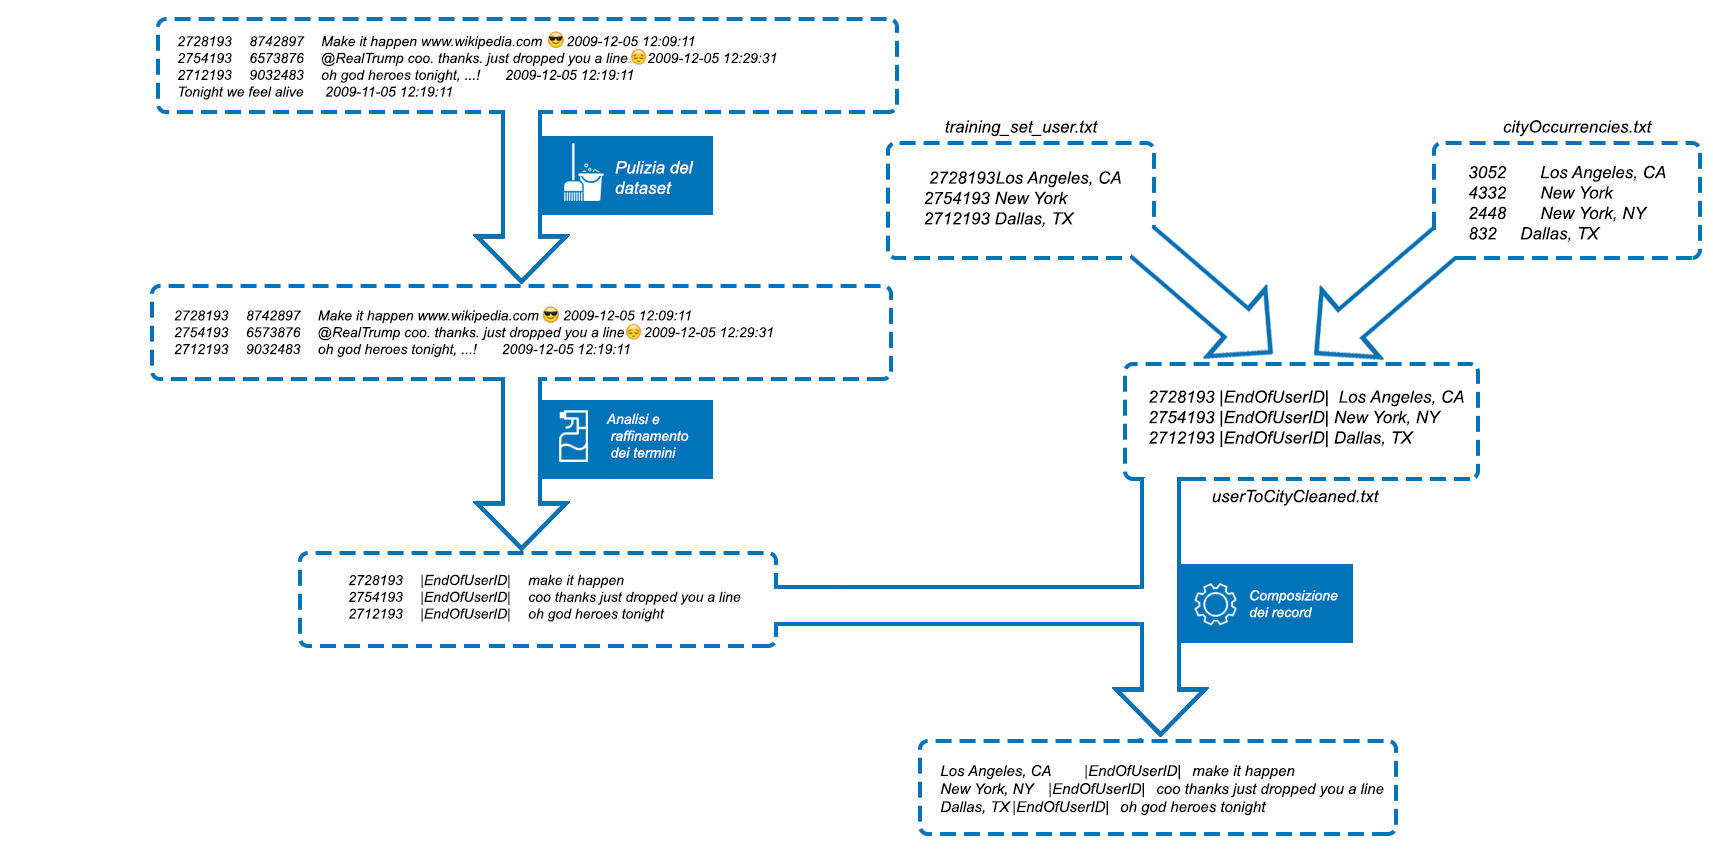
\includegraphics[width=16cm,height=8.65cm]{figure/matita2.png}
  \caption{Nella figura vengono mostrate le dipendenze individuate tramite la libreria di Stanford. Gli nmod rilevanti, cerchiati in verde, sono quelli che presentano diversi dependent. nmod:of viene quindi scartato in quanto presenta una sola dependent.}
\end{figure*}  


\subsection{Parsing}

La prima fondamentale differenza con le implementazioni proposte dallo studente Tanzi risiede nell'utilizzo dello \textit{Jazzy Spell Checker}. Essenzialmente si tratta  di un modulo che corregge le parole in input non scritte correttamente associandole a termini simili. \\ Ad esempio il termine \textit{boook} verrebbe associato al corrispettivo \textit{book}. \\ Questo processo  introduce un overhead considerevole, dovendo effettuare un confronto tra ciascuna delle $9 M$ di parole nel dataset con $350K$ record nel dizionario. Oltre al notevole costo computazionale si tratta di un processo che esclude termini che potrebbero essere potenzialmente rilevanti nell'intero processo di geolocalizzazione. Questo \'e dovuto principalmente alla presenza di termini dello slang che non fanno parte del dizionario: si \'e quindi deciso di non utilizzare tale modulo.\\ Il processo di parsing si articola in 3 fasi differenti:

\begin{enumerate}
\item Pulizia del dataset
\item Analisi e raffinamento dei termini
\item Composizione dei record 
\end{enumerate}


La fase di pulizia del dataset si occupa di scartare tutti quei tweet che non sono nel formato richiesto, ovvero \textit{id utente, id tweet, testo}. \\Il numero di tweet che non risultavano formattati correttamente e quindi scartati dal primo filtro \'e di circa \textbf{100K}.\\La fase successiva, quella dell'analisi e del raffinamento dei termini, ha invece lo scopo di eliminare il contenuto che non \'e di interesse nel processo di geolocalizzazione. \\In particolare, vengono scartati:
\begin{enumerate}
\item Indirizzi email 
\item Siti
\item Hashtag
\item Tag
\item Parole contententi caratteri non ASCII
\item Caratteri singoli
\item Tweet duplicati
\end{enumerate}

Alla fine di questa fase vengono scartati ben $170K$ tweet. I rimanenti subiscono un' ulteriore traformazione consistente in un join con  le coppie \textit{utente-citt\'a}. \\Come accennato in precedenza, nel dataset non tutti gli utenti sono correttamente geotaggati.\\ Il problema pi\'u frequente consiste nel fatto che alcune citt\'a sono sprovviste della sigla dello Stato: per ovviare a questo problema si \'e adottata la soluzione di assegnare alle citt\'a lo stato corrispondente alla citt\'a omonima e pi\'u popolosa. Anche in caso di citt\'a malformattate, come ad esempio  \textit{New York, New York}, il secondo elemento viene rimosso in favore del relativo Stato. 

\subsection{TfIdf}

Il processo di geolocalizzazione avviene sulla base del calcolo del \textit{Tf-Idf} delle parole all'interno dei tweet. Intuitivamente parole che sono utilizzate molto in una citt\'a e poco nelle altre sono  preziosi indicatori. \\La formula utilizzata differisce leggermente da quella presente nel paper, ed \'e la seguente: $$tf_{ij}=	\frac{f_{ij}}{max_k	\left \{ f_{kj} \right \}	}$$

$$idf_i= log_{a}\left ( \frac{N}{df_i} \right )$$
In un primo momento nel calcolo del \textit{tf-idf} sono state prese in considerazione tutti i termini presenti nei tweet, implicando un tempo di esecuzione di circa $4h$. Dopo un'attenta analisi \'e emerso che molti dei termini presenti, circa il $90\%$, si presentavano meno di 50 volte all'interno dell'intero dataset. Escludendo le parole in questione e senza avere impatti negativi sull'accuratezza \'e stato possibile abbassare il tempo di esecuzione a $15 min$. 


\subsection{Validazione}

Il modulo di geolocalizzazione \'e stato validato sul dataset di test utilizzato in \textit{You Are Where You Tweet}. I dati in input sono stati processati come illustrato in Sez. 3.1. 
\begin{table}[t]
\caption{Esempio dei record utilizzati nel processo di validazione}
\begin{center}
\label{table_ASME}
\begin{tabular}{c l l}
& & \\ % put some space after the caption
\hline
Word & City Coordinates &  Tf-Idf \\
\hline
love & 44.9800000, -93.2636111 & \ 0,03\\
peace &  47.8211111, -122.3138889 & \ 0,01 \\
morales & 25.7738889, -80.1938889 & \ 0,027 \\

\hline
\end{tabular}
\end{center}
\end{table}

Un aspetto rilevante di questa fase \'e il calcolo delle distanze tra coordinate relative a citt\'a diverse. Nell'implementazione dello studente Tanzi era previsto un uso massiccio dell'API \textit{Google Geocoder} per determinare le coordinate corrispondenti a una citt\'a e poi calcolare le distanze. L'utilizzo dell'API \'e per\'o limitato ad un massimo di $2500$ richieste giornaliere e per questo motivo un approccio basato su continue interrogazioni \'e destinato a interrompersi. L'implementazione corrente sfrutta invece una mappa esistente di tipo \textit{citt\'a, coordinate} e inoltra richieste all'API soltanto nel caso in cui il record d'interesse non \'e presente. Tale implementazione sostiene anche l'utilizzo dello streaming per il retrieve di nuovi dati. Per il calcolo della distanza tra due coordinate abbiamo fatto uso della seguente formula: 
$$d=  \arccos{\left ( \sin{\left (A_1 \right )} \cdot \sin{\left (A_2 \right )} + \cos{\left (A_1 \right )} \cdot \cos{\left (A_2 \right )} \cdot \cos{\left (B_2 - B_1 \right )} \cdot \lambda \right ) }$$

e coordinate di latitudine $A_i$, longitudine $B_i$ e $\lambda=6371$. 

\section{Risultati}

Nel valutare l'accuratezza del modulo di geolocalizzazione si sono seguiti diversi approcci. \\Una prima verifica \'e stata effettuata focalizzandoci sul singolo messaggio: a ciascun tweet vengono associate le citt\'a pi\'u probabili sulla base del \textit{Tf-Idf} di ciascuna parola. In modo particolare, ciascuna parola \'e collegata a una lista di citt\'a con i relativi \textit{Tf-Idf}; parola per parola tali punteggi verranno aggregati. In questo modo viene stilata una classifica delle localit\'a pi\'u probabili di provenienza del tweet. L'accuratezza ottenuta selezionando la prima citt\'a \'e stata di circa il $3\%$. Aumentando fino a $5$ il numero di citt\'a candidate si \'e invece raggiunta un'accuratezza del $20\%$ Questa soluzione differisce dalle soluzioni presentate nel paper di riferimento, che invece focalizzano il processo di valutazione sul \textit{corpus tweet} dell'utente. \\I risultati presentati nell'articolo per questo tipo di valutazione attestano   
valori di accuratezza compresi tra il $10$ e il $47\%$.  \\Il nostro approccio per la geolocalizzazione di un utente prevede come prima fase l'accorpamento di tutti i suoi tweet. Quindi, a partire da questo testo, viene calcolato il relativo \textit{Tf-Idf} che risulta molto pi\'u significativo rispetto a quello ottenuto dal singolo tweet. I risultati ottenuti in questo caso sono compresi tra il $12\%$ e il $37\%$. Una completa comparazione dei risultati \'e mostrata in Tab.2. \'E interessante notare che le stopword sono in realt\'a utili per una corretta geolocalizzazione.


\begin{table}[h]
\caption{Confronto dei risultati ottenuti con quelli presenti nel paper.}
\begin{center}
\label{table_ASME}
\begin{tabular}{c l l l l l}
& & \\ % put some space after the caption
\hline
Method & AC &  AC@2 &  AC@3 & AC@4 &  AC@5 \\
\hline
Baseline paper &  10,1\% &  37,5\% &  42,5\% & & 47,6\% \\
Baseline  &  12,5\% &    &  26,2\% & 32,4\% & 36,2\% \\
+ Stopword &   &    &  &  & 32,3\% \\

\hline
\end{tabular}
\end{center}
\end{table}
\end{document}
